% In your report, answer the following questions.
% A. Understand and analyze each calibration step from the camera calibration toolbox for Matlab
% B. Show the calibration results for the initialization and non-linear optimization steps
% C. Visualize the re-projection errors and extrinsic parameters (3D plot)


\section{Calibration steps}

Assuming we already have the required images for calibration, the first step is
to read the images into the Matlab, so that the calibration toolbox can use
them. After that, we can start with the grid corner extraction.

We go through each image, and manually mark the extreme corners of the
calibration pattern, which is a grid of black and white rectangles, whose
dimensions are known. Using those corners, the toolbox is able to estimate the
boundary of the calibration grid, and using that boundary is able to estimate
the corners of all the individual rectangles.

At this point, some of the corners might be wrong. This is because of camera
distortion. We can manually correct for the distortion at this point, but I
chose to let the toolbox calculate the distortion automatically.

After extracting the preliminary corners, it's time for the main calibration
step. The first step is the initialization. This step calculates a closed form
solution for the camera parameters, and it doesn't take lens distortion into
account. That's why we only obtain the focal lenght and principal point
parameters.

To get the lens distortion, we run the non-linear optimization algorithm, which
minimizes the total reprojection error. It takes into account all the camera
parameters in this optimization. From this step we obtain the lens distortion
and pixel error. We also obtain the uncertainties for all the parameters.

However, due to not manually correcting for the lens distortion on the first
run, our results are not perfect. To get better results, we can (automatically)
recompute the grid corners, and run the calibration again with those recomputed
corners.



\section{Results}

After the initialization step of the calibration, we only have the
\textbf{focal length} and \textbf{principal point} intrinsic parameters. They
are presented in the table~\ref{tab:init_param}


\begin{table}[h]
  \centering
  \caption{Calibration parameters after initialization}\label{tab:init_param}
  \begin{tabular}{l N{5}{2} N{5}{2}}
    \toprule

    Focal length:       &   670.66552   &   670.66552   \\

    \midrule

    Principal point:    &   319.50000   &   239.50000   \\

    \bottomrule
  \end{tabular}
\end{table}

After the optimization we get more results; In addition to the recalculated
focal lenght, principal point, and their uncertainties, we get the camera
\textbf{distortion} and \textbf{pixel error} (and their uncertainties). The
final results (after grid corner recomputation and a second calibration) can be
found in the table~\ref{tab:optim_param}

\begin{table}[h]
  \centering
  \caption{Calibration results after optimization (with uncertainties)}\label{tab:optim_param}
  \begin{tabular}{l N{5}{2} N{5}{2} N{5}{2} N{5}{2} N{5}{2}}
    \toprule

    Focal length:       &   657.48040   &   657.93987   \\
    +/-                 &   0.37682     &   0.40757     \\

    \midrule

    Principal point:    &   302.57943   &   242.35496   \\
    +/-                 &   0.74700     &   0.73371     \\

    \midrule

    Distortion:  &   -0.25430 & 0.11808 & -0.00031 & -0.00009 & 0.00000 \\
    +/-          &   0.00298  & 0.01268 & 0.00016  & 0.00016  & 0.00000 \\

    \midrule

    Pixel error:        &   0.12547     &   0.11997 \\

    \bottomrule
  \end{tabular}
\end{table}

The camera \textbf{skew} isn't calculated, because modern cameras are assumed
to have rectangular pixels. This is the default setting in the calibration
toolbox. Figure~\ref{fig:reprojection} has a visualization of the reprojection
error, and figure~\ref{fig:extrinsic} has the extrinsic parameters in a 3D plot.


\begin{figure}[h]
  \centering
  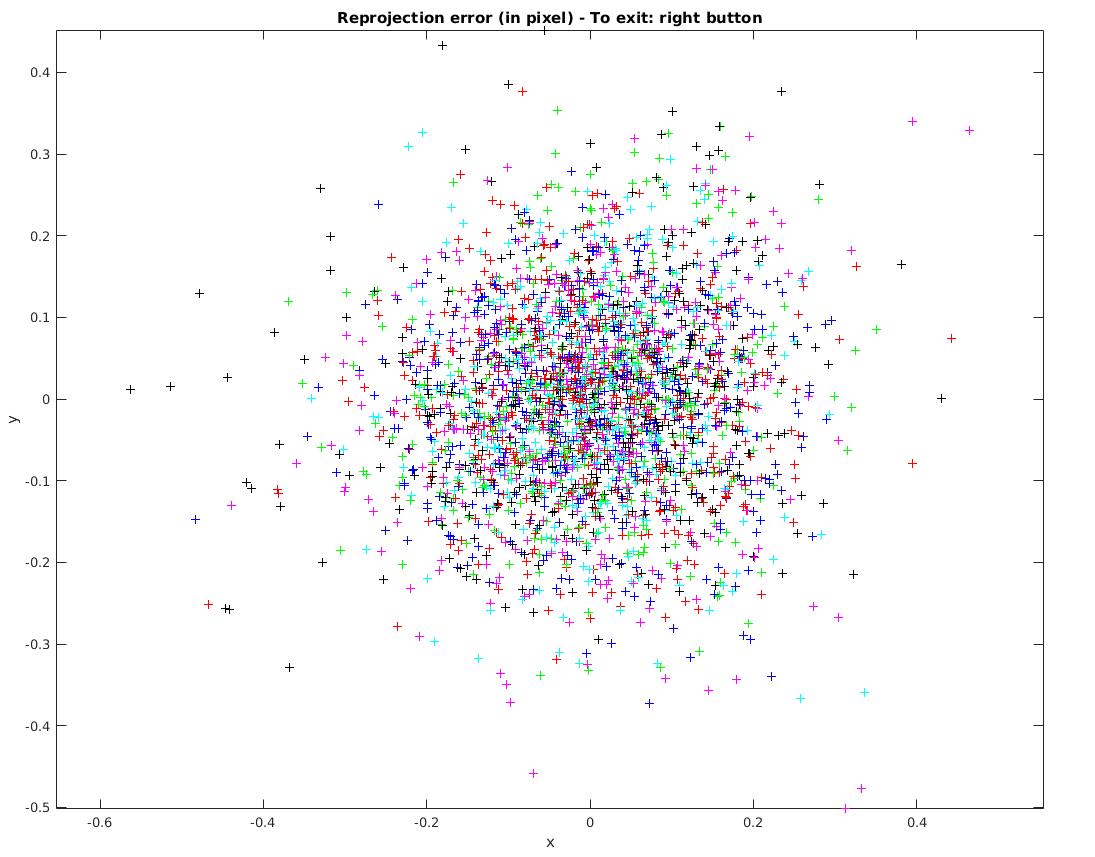
\includegraphics[width=0.8\linewidth]{reprojection_error_recomp}
  \caption{Visualization of the reprojection error}\label{fig:reprojection}
\end{figure}


\begin{figure}[h]
  \centering
  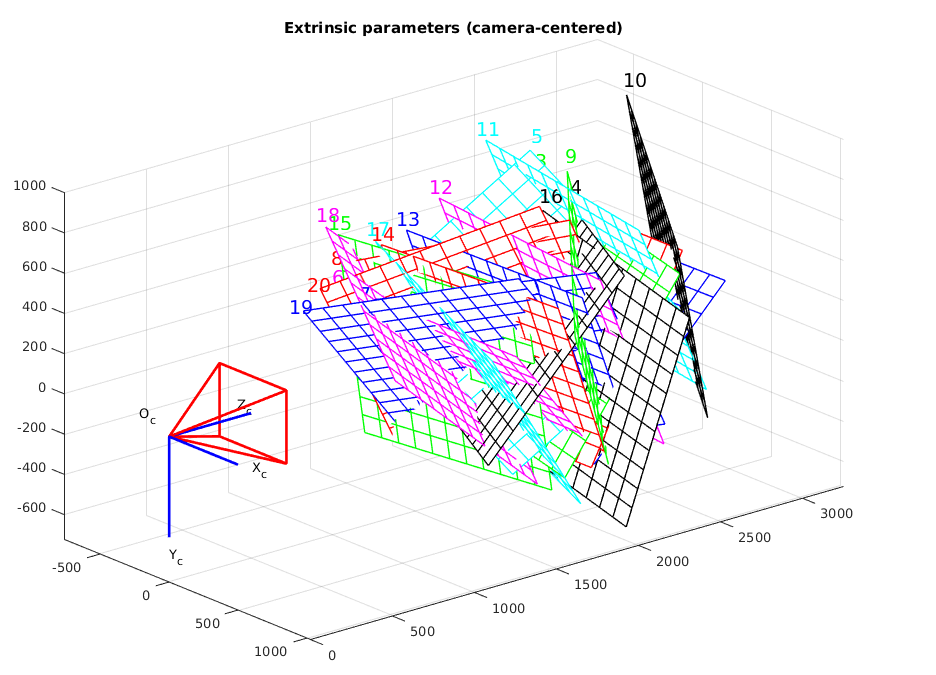
\includegraphics[width=0.8\linewidth]{extrinsic_cam_centered_recomp}
  \caption{Visualization of extrinsic parameters}\label{fig:extrinsic}
\end{figure}

\section{Explanation of parameters}

% TODO: explain the concepts of focal lenght, principal point, distortion and
% pixel error
% TODO:maybe explain the reprojection error and extrinsic parameters, or like,
% whats the point about visualizing them
\begin{description}

  \item[Focal length]           töttöröö

  \item[Principal point]        tlttl

  \item[Skew coefficient]       tasda

  \item[Distortions]            asdasd

  \item[Pixel error]            asdafdf

  \item[Extrinsic parameters]   asdasd

  \item[Reprojection error]     asdafdf

\end{description}
